% !TeX encoding = UTF-8
% !TeX spellcheck = it_IT
% !TeX root = main.tex

\section{Componenti aggiuntive}
Il sistema oltre a fornire i servizi di base necessari a soddisfare l'obiettivo prefissato definito nella sezione \ref{scopo}, presenta alcune funzionalità aggiuntive atte a migliorare l'esperienza con il sistema. Tra queste funzionalità aggiuntive, le principali sono:
\begin{itemize}
	\item Modulo di spiegazione
	\item Interfaccia grafica Java
	\item Rappresentazione visuale delle spiegazioni tramite graphviz
\end{itemize}
Di seguito verrà fatta una breve descrizione per ogni funzionalità.

\subsection{Modulo di spiegazione}
\label{spiega}
Il sistema, una volta terminata l'elaborazione e mostrato a video i risultati del tag, da la possibilità all'utilizzatore di capire come è stato possibile etichettare quel gruppo di parole in un determinato tag. Per fare ciò, durante l'elaborazione, il sistema man mano che cerca di etichettare un particolare tag (ad esempio \emph{Persona}), asserisce oltre ai vari IDDoc, ListaPrecedenti, ListaSuccessivi, etc. , anche la spiegazione di come si è raggiunto quel particolare tag.

Ad esempio, in caso di tag di persone, all'interno del predicato \emph{tag\_persone}, sarà presente anche:

\begin{prologcode}
 tag_persona(C, N) :-
   ...
   atomic_list_concat(['[PERSONA] Presenza nel documento di:',C,N],
                      ' ',Spiegazione),
   ...
   assertTag(persona(C, N),IDDoc, ListaPrecedenti, ListaSuccessivi,
            Spiegazione, Dipendenze).
\end{prologcode}

Successivamente, qualora l'utente dovesse richiedere la spiegazione di un particolare tag, il sistema, indipendentemente dall'interfaccia utilizzata (per i diversi tipi di approcci interattivi vedere cap. \ref{Interaction}), non farà altro che richiamare il predicato \emph{spiega\_tutto/2} il cui compito sarà quello di recuperare tutte le spiegazioni dei vari sottotag che compongono il tag di cui si vuole ottenere la spiegazione.
Ad esempio, se nel documento è presente una frase del tipo : ``\emph{... Richiesta in via chirografaria di 2000 \officialeuro ...}'' , in questo caso il sistema creerà un tag \emph{richiesta\_valuta(2000, euro, chirografario)}.

Qualora volessimo sapere il come è stato creato questo tag, il sistema risponderà nel seguente modo:

\begin{verbatim}
[RICHIESTA VALUTA] Presenza nella stessa frase della valuta 2000
                   euro e del termine chirografaria
[TIPO_RICHIESTA] Presenza nel documento del termine chirografaria
[VALUTA] Presenza nel documento del numero 2000 seguito dal 
         simbolo €

\end{verbatim}
\subsection{Interfaccia grafica Java}
Tra le feature aggiuntive offerte dal sistema, vi è la presenza di un'interfaccia grafica creata in Java utile al fine di poter migliorare l'usabilità del sistema permettendone l'utilizzo anche a chi non è molto pratico di interfacce a linee di comando. Nel capitolo \ref{Interaction} verrà descritto in dettaglio come si presenta l'interfaccia grafica e un suo esempio di interazione. 
Per permettere la realizzazione delle interfacce grafiche in Java è stato, inoltre, necessario far comunicare Prolog con Java in modo tale da garantire uno scambio di informazioni tra i due sistemi; per fare ciò sono state utilizzate due librerie Java nate per questo scopo quali JPL e InterProlog di cui si parlerà approfonditamente rispettivamente nelle sezioni \ref{JPL} e \ref{InterProlog}.
\subsection{Rappresentazione visuale tramite graphviz}
\nocite{gansner2006drawing}
\nocite{wiki:Graphviz}
Un'ulteriore feature offerta dal sistema è quella inerente al modo con cui visualizzare le spiegazioni dei tag che il sistema ha creato; in particolare, oltre alla spiegazione testuale cosi come mostrata nella sezione \ref{spiega}, il sistema offre un'immagine che mostra in maniera grafica come è stato ottenuto il tag.
Prendendo come esempio il tag \emph{richiesta\_valuta} descritto nella sezione \ref{spiega}, la visualizzazione grafica di quel tag sarà:

\begin{figure}[H]
	\centering
	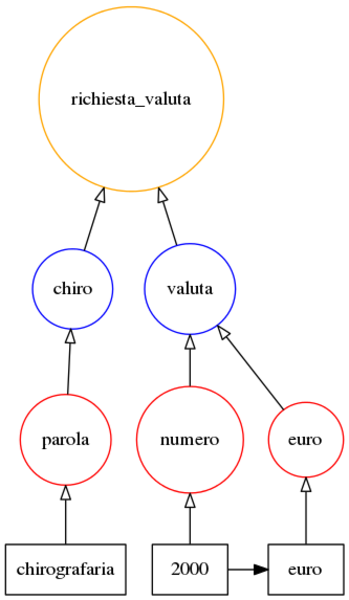
\includegraphics[width=0.5\textwidth]{img/tagRichiesta.png}
	\caption{Esempio spiegazione richiesta\_valuta}
\end{figure}

Per poter ottenere un grafico di questo tipo, è stato necessario utilizzare un programma open source chiamato \emph{Graphviz}\footnote{Scaricabile dal sito \url{http://www.graphviz.org/}} (abbreviazione di Graph Visualization Software), il quale è in grado di disegnare grafi descritti nel linguaggio \emph{DOT}.

Il linguaggio \emph{DOT} è un linguaggio di descrizione di grafi in plain text, la cui peculiarità principale risulta essere la facilità d'uso sia da parte dell'essere umano che dalla macchina. I grafi descrivibili da questo linguaggio possono essere sia grafi orientati che non; nel nostro caso è stato necessario garantire la direzionalità dell'arco.
\clearpage
Un esempio di codice dot per descrivere un grafo orientato (\emph{V},\emph{E}), dove 
$$V = \left\{ a,b,c \right\} $$
$$E = \left\{ \left( a,b \right) , \left( b,c \right) , \left( b,d \right) \right\} $$
è il seguente:

\begin{verbatim}
	digraph graphExample {
	    a -> b -> c;
	    b -> d;
	}
\end{verbatim}
Dove la parola chiave \emph{digraph} indica che il grafo che si andrà a creare sarà orientato (Directed), mentre \emph{graphExample} sarà il nome del grafo da creare.
Una volta creato il file .dot sarà necessario processarlo dall'omonimo programma al fine di poter ottenere l'immagine in formato PNG da poter visualizzare.
Il comando da terminale da dover usare per la creazione dell'immagine in formato PNG sarà il seguente:
\begin{verbatim}
  dot -Tpng ./graphExample.dot > ./graphExample.png
\end{verbatim}

L'output dell'immagine creata dal dot sarà:
\begin{figure}[H]
	\centering
	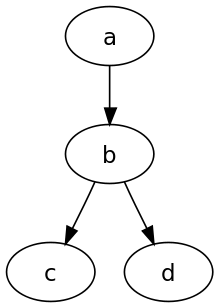
\includegraphics[width=0.4\textwidth]{img/220px-DotLanguageDirected.png}
	\caption{Esempio di grafo dot}
\end{figure}